\documentclass[a4paper]{article}

%% Language and font encodings
\usepackage[portuges]{babel}
%\usepackage{fontspec}

%% Sets page size and margins
\usepackage[a4paper,top=3cm,bottom=2cm,left=3cm,right=3cm,marginparwidth=1.75cm]{geometry}

%% Useful packages
\usepackage{amsmath,amsthm,amssymb,amsfonts}
\usepackage{graphicx}
\usepackage[colorinlistoftodos]{todonotes}
\usepackage[colorlinks=true, allcolors=blue]{hyperref}
\usepackage{subfig}
\usepackage{float}



\newcommand{\R}{\mathbb{R}}
\newcommand{\N}{\mathbb{N}}
\newcommand{\Z}{\mathbb{Z}}
\providecommand{\C}{\mathbb{C}}

\theoremstyle{definition}
\newtheorem{defin}{Definição}

\theoremstyle{plain}
\newtheorem{theorem}[defin]{Teorema}
\newtheorem{corollary}[defin]{Corolário}



\title{Laboratório de CEME - Lab 2\\Simulação de um sistema eletromecânico: Contatora}

\author{Cleiton M. Freitas\\
}

\date{}

\begin{document}
\maketitle

%\begin{abstract}
%Your abstract.
%\end{abstract}

%%%%%%%%%%%%%%%%%%%%%%%%%%%%%%%%%%%%%%%%%%
%%%%%%%%%%%%%%%%%%%%%%%%%%%%%%%%%%%%%%%%%%
%%%%%%%%%%%%%%%%%%%%%%%%%%%%%%%%%%%%%%%%%%
\section{Objetivo}

O objetivo desta experiência é montar a simulação de um sistema eletromecânico simples, o sistema de uma contatora. Para isso, combinaremos os métodos aprendidos na aula teórica com a metodologia de simulação utilizada no \textbf{LAB 1}.

%%%%%%%%%%%%%%%%%%%%%%%%%%%%%%%%%%%%%%%%%%
%%%%%%%%%%%%%%%%%%%%%%%%%%%%%%%%%%%%%%%%%%
%%%%%%%%%%%%%%%%%%%%%%%%%%%%%%%%%%%%%%%%%%
\section{A contatora}


Uma contatora é um sistema geralmente utilizado como chave eletromecânica. Ou seja, quando injetamos corrente na sua bobina, a parte móvel do núcleo é atraída para uma posição de forma a fechar ou abrir um circuito. Uma boa descrição do funcionamento de uma contatora é encontrada em \cite{Faustino2020} e \cite{meletrica2014}.


A Figura~\ref{fig:contatora} apresenta o diagrama com dois estados de uma contatora similar àquela explicada em \cite{Faustino2020,meletrica2014}. Como pode ser observado, a contatora possui um núcleo dividido em duas partes, uma delas fixa e outra móvel, uma bobina e uma mola. A bobina é enrolada em um carretel, não representado aqui, que serve de suporte para a mola. Assim, o formato da bobina se materá inalterado independentemente da condição da mola. Quando a corrente na bobina é nula, a mola empurra a parte móvel do núcleo para longe da parte fixa. Quando injetamos corrente, a força magnética produzida gera uma atração entre as diferentes partes do núcleo e, consequentemente, a mola é contraída. A Figura~\ref{fig:contatora:comI} apresenta o caso extremo, onde as duas partes do núcleo se tocam, mas a compressão da mola (e a distância entre as partes do núcleo) vai depender da quantidade de corrente injetada na bobina.
%
\begin{figure}[H]
\centering
\subfloat[$i = 0$]{
\label{fig:contatora:semI}
\includegraphics[width=0.48\linewidth]{./figuras/contatora_0}
}
\subfloat[$i \neq 0$]{
\label{fig:contatora:comI}
\includegraphics[width=0.48\linewidth]{./figuras/contatora_1}
}
\caption{Esquema de uma contatora}
\label{fig:contatora}
\end{figure}

 


%%%%%%%%%%%%%%%%%%%%%%%%%%%%%%%%%%%%%%%%%%
%%%%%%%%%%%%%%%%%%%%%%%%%%%%%%%%%%%%%%%%%%
%%%%%%%%%%%%%%%%%%%%%%%%%%%%%%%%%%%%%%%%%%
\section{Desenvolvimento das Simulações}


Como no caso anterior, a simulação deverá ser capaz de calcular a resposta dinâmica do sistema para uma conjunto de variáveis. Neste caso, a corrente da bobina ($i$), a posição ($x$) e a velocidade ($v$) da parte móvel do núcleo. A Figura~\ref{fig:cotas} apresenta um novo diagrama da contatora, desta vez omitindo a mola para facilitar a análise da parte magnética. Observe que todos os diagramas representam a vista superior da contatora, ou seja, o sistema está deitado e não sofre atuação da força da gravidade. Além disso, as duas partes do núcleo são simétricas, ou seja, as cotas da parte fixa (inferior) são iguais as da parte móvel (superior).



\begin{figure}[!htb]
\centering
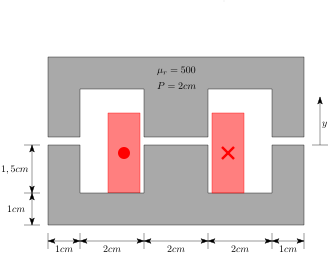
\includegraphics[width=0.85\linewidth]{./figuras/contatora_cotas}
\caption{Diagrama da contatora com as devidas cotas}
\label{fig:cotas}
\end{figure}


Como esperado, para simular a dinâmica do sistema, deveremos obter três equações diferenciais\footnote{Embora tenha escrito $f_1$, $f_2$ e $f_3$ com três variáveis, $x$, $i$ e $v$, nem todas funções terá as três variáveis}:

\begin{equation}
\frac{d i}{dt} = f_1 (x,i,v)
\end{equation}

\begin{equation}
\frac{d x}{dt} = f_2 (x,i,v)
\end{equation}

\begin{equation}
\frac{d v}{dt} = f_3 (x,i,v)
\end{equation}



Para obter a equação diferencial da corrente, devemos seguir um procedimento parecido ao utilizado no \textbf{LAB 1}. Ou seja, devemos obtê-la a partir da manipulação da equação de malha do circuito elétrico da Figura~\ref{fig:mag}. Neste circuito, $V_{in}$ é uma tensão constante que alimentará a bobina e $e$ é a tensão induzida da bobina.


\begin{figure}[!htb]
\centering
\includegraphics[width=0.50\linewidth]{./figuras/circuito_bobina}
\caption{Interface eletromagnética do sistema}
\label{fig:mag}
\end{figure}


Para obter as equações mecânicas, ou seja, as equações diferenciais de $x$ e $v$, devemos recorrer aos nossos conhecimentos de física básica. Assim:

\begin{equation}
m a = \displaystyle \sum \text{Forças}
\end{equation}
%
onde $m$ e $a$ são a massa e a aceleração da parte móvel. Considerem três forças no sistema, a força magnética, a força da mola e a força do atrito aerodinâmico ($-b v$, onde $b$ é o coeficiente de atrito). Lembrem que as equações devem estar em função de $x$, $v$ e $i$. Ou seja, o $a$ não pode aparecer. A equação diferencial de $x$ é direta, ou seja, é uma definição geral da cinética. 



%%%%%%%%%%%%%%%%%%%%%%%%%%%%%%%%%%%%%%%%%%%
%%%%%%%%%%%%%%%%%%%%%%%%%%%%%%%%%%%%%%%%%%
%%%%%%%%%%%%%%%%%%%%%%%%%%%%%%%%%%%%%%%%%%
\section{Tarefas Iniciais}


\begin{enumerate}
	\item Obter a indutância do circuito em função da posição $x$ da parte móvel do núcleo.
	\item Calcular a força magnética em função da posição $x$ e da corrente $i$.
	\item Obter a equação diferencial de corrente
	\item Obter a equação diferencial da posição $x$
	\item Obter a equação diferencial da velocidade $v$
\end{enumerate}





%%%%%%%%%%%%%%%%%%%%%%%%%%%%%%%%%%%%%%%%%%%
%%%%%%%%%%%%%%%%%%%%%%%%%%%%%%%%%%%%%%%%%%
%%%%%%%%%%%%%%%%%%%%%%%%%%%%%%%%%%%%%%%%%%
\section{Dados do Problema}





\begin{table}[H]
\centering
\caption{Parâmetros da Contatora}
\begin{tabular}{ccc}
\hline
\textbf{Parâmetro} & \textbf{Notação} & \textbf{Valor}\\ \hline
Massa da parte móvel & $m$ & 100$g$\\
Coeficiente de atrito aerodinâmico & $b$ & 0.2 $kg/s$\\
Número de Espiras & $N$ & 1000\\
Resistência da Bobina & $R$ & 1$k\Omega$\\
Constante de força da mola & $k$ & 1 $kg/s^2$\\ 
Condição a qual a mola não está estressada & $x_r$ & 1$cm$\\ 
Tensão de alimentação & $V_{in}$ & -\\ 
\hline
\end{tabular}
\end{table}



%%%%%%%%%%%%%%%%%%%%%%%%%%%%%%%%%%%%%%%%%%%
%%%%%%%%%%%%%%%%%%%%%%%%%%%%%%%%%%%%%%%%%%
%%%%%%%%%%%%%%%%%%%%%%%%%%%%%%%%%%%%%%%%%%
\section{Casos Teste}

Os casos teste serão divididos em quatro partes: a parte 1  servirá simplesmente para analisar a parte mecânica do sistema; as partes 2 e 3 servirão para analisar as limitações da analise; e a parte 4 para comparar resultados. Em todos os casos utilizaremos vetores com 10000 pontos. 




%%%%%%%%%%%%%%%%%%%%%%%%%%%%%%%%%%%%%%%%%%
\subsection{Parte 1: parte mecânica isolada}


\begin{itemize}
\item Configure a tensão de alimentação para 0V (zero), assim não teremos interferência da parte elétrica;

\item Configure a corrente inicial e a velocidade inicial para 0 (zero);

\item Configure a posição inicial para $0.8x_r$, ou seja, a condição em que a mola está ligeiramente comprimida;

\item Antes de similar, tente imaginar o que deveria acontecer com o sistema;

\item Execute a simulação para 10s;

\item O que você imaginou aconteceu nos resultados?

\end{itemize}




%%%%%%%%%%%%%%%%%%%%%%%%%%%%%%%%%%%%%%%%%%
\subsection{Parte 2: limites da análise - precisão}

Primeiramente:

\begin{itemize}
\item Configure a tensão de alimentação para 20V;

\item Configure a corrente inicial e a velocidade inicial para 0 (zero);

\item Configure a posição inicial para $x_r$, ou seja, a condição em que a mola está relaxada;

\item Antes de similar, tente imaginar o que deveria acontecer;

\item Execute a simulação para 10s;

\item O que você imaginou aconteceu nos resultados?

\item analise em especial o comportamento da corrente e da posição. Talvez seja necessário dar uma zoom no gráfico de corrente. Use o comando \verb|plt.xlim(...)| para isso. 
\end{itemize}


Em seguida, repita a simulação anterior, mas desta vez considerando um tempo final de simulação de $10ms$. Que diferença é observado especialmente com a corrente? Porque ocorreu esta diferença?


%%%%%%%%%%%%%%%%%%%%%%%%%%%%%%%%%%%%%%%%%%
\subsection{Parte 2: limites da análise - condições impossíveis}

Repita o item anterior, desta vez considerando 35V de alimentação e um tempo de simulação de 20s. O que aconteceu com os resultados e como você pode interpretar isso?



%%%%%%%%%%%%%%%%%%%%%%%%%%%%%%%%%%%%%%%%%%
\subsection{Parte 4: Testes}

Faça 3 simulações de 10s, uma com a tensão de alimentação de 10V, outra 20V e outra 34V. Anote os valores de regime permanente da corrente e da posição e use-os para para calcular a força magnética em cada um dos casos.



\bibliographystyle{ieeetr}
\bibliography{referencias}




\end{document}